\chapter{Experiment Design}\label{chapter:Experiment}

\section{Experiment Overview}
This study tests the capabilities of modern vision language models (VLMs) 
to see how well they can move beyond pixel faithfulnuss and automatically
produce accessible front-end code. 
Figure xy demonstrates our automatic Image-to-Code pipeline where an 
image with instructions is given as input and standards-compliant HTML/CSS 
is generated by the models.
The output is then analyzed within multiple stages to evaluate visual 
and structural similarity, as well as \textit{WCAG 2.2} compliance.\newline
In order to account for the probabilistic nature of LLMs, each experiment 
will be repeated within 3 experiment runs.

\begin{figure*}[p]
  \centering
  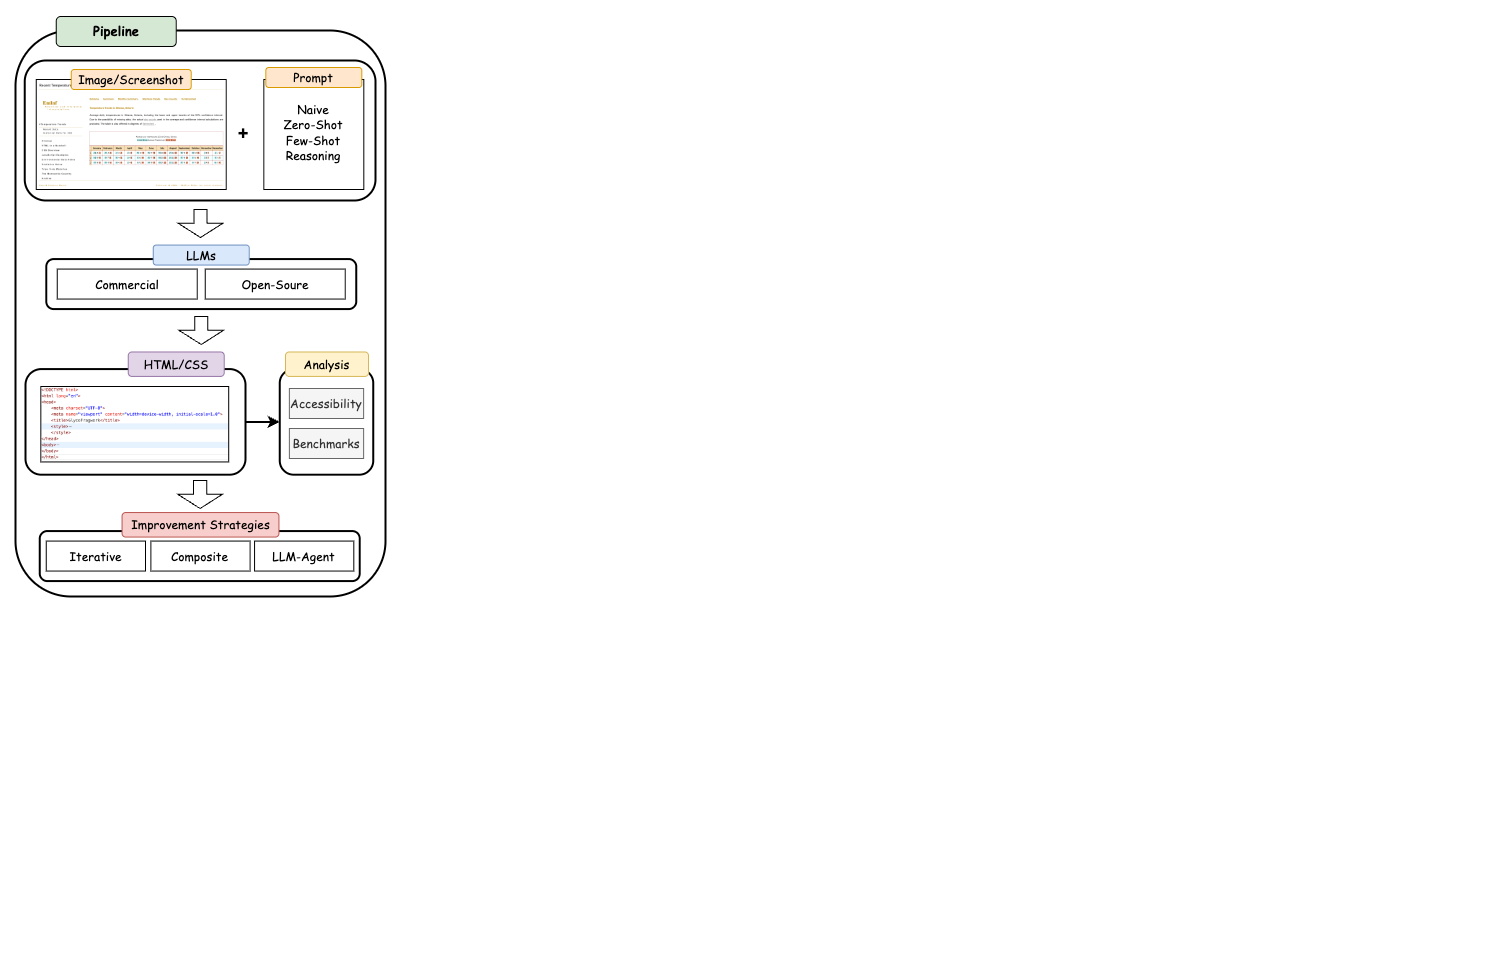
\includegraphics[width=\textwidth]{figures/pipeline.png}
  \caption{Experiment Pipeline}
  \label{fig:pipeline}
\end{figure*}


\subsection{Model Selection}
The selection of the LLMs is a decisive factor for the interpretation of the results.
To see the diffences of performance, we decided to use different types of 
state-of-the-art models. All have native vision capabilities, but they differentiate 
in size, architecture and target audience.
In order to provide a general picture, we identified two model groups of interest:
\begin{itemize}
  \item \textbf{Commercial:} Big, commercial models build the foundation of our tests.
    We use \textit{ChatGPT-4o} and \textit{Gemini Flash 2.0} as representatives of this group.
    They have not been specifically trained for Image-to-Code tasks, but prior papers 
    already show promising results in this field.
  \item \textbf{Open-Source:} Small, open-source models build the second group. 
    While they are signifant smaller than the commercial models, theoretically they 
    could be hosted by anyone and therefore might be more accessible for the public.
    The representative of this group is \textit{Qwen 7B vl}.
\end{itemize}

\section{Prompting Techniques}
To understand the models' capabilities to generate accessible code, we test
them with different prompting techniques (full text in appendix). Each 
prompt provides the screenshot (B64 decoded) and a description of the
task.\newline
Prior research has shown that more 
advanced prompting techniques can help to improve the generation of robust and 
accurate code.
The wording of the prompts is similar to the one of prior research~\parencite{suh2025accessiblecode, xiao2024interaction2code}.
The content is the same while we have enriched the prompts with more details.\newline

\subsection{Naive}
The naive approach only instructs the LLMs to accurately fulfill Image-to-Code tasks
without mentioning accessibility in its prompt. This shows how state-of-the-art 
LLMs perform in generating accessible code naturally without instructing it to 
do so.

\subsection{Zero-Shot}
The zero-shot approach resembles the naive approach in terms of the Image-to-Code
instructions. However, here the LLMs are explicitly instructed to obey the WCAG 
2.2 standards. The prompt does not contain examples, however it emphasizes 
accessibility by reminding it about the WCAG standards including a link to 
official WCAG standards.

\subsection{Few-Shot}
The few-shot approach resembles the zero-shot prompt, however it is enriched with 
explicit examples to support the LLM to generate more accessible code. 
Since the number of possible examples is too large, we decided to provide examples 
for only 8 of the most common accessibility violations (e.g. Missing Alt-Text, 
Color Contrast). 
For this approach, we have followed the structure of previous 
works~\parencite{suh2025accessiblecode}.
The structure of the examples contains the rule's name, a description, a
correct example and a wrong counter example. If possible, the examples 
were taken from the official W3C website~\parencite{wcag21}.

\subsection{Chain-of-Thought}
The chain-of-thought prompt is used to let the LLMs reason about the task and possible 
accessibility problems within the generation. Similar to prior work, we use 
the reasoning instructions \"Let’s think step by 
step.\" and instruct the model to output its reasoning comments which 
are then stripped in a pre-processing step.~\parencite{chae2024thinkexecute}.



\section{Improvement Strategies}
To solve the limitations of current prompting techniques, we test three 
advanced improvement strategies that explicitly correct accessibility 
violations. One is an iterative approach that uses the 
feedback from accessibility tools in an iterative manner to improve the code.
The second is a composite approach which combines 
pre-processing and post-processing techniques to improve the LLMs' output.
The last approach is a multi-agent approach that uses further 
state-of-the-art LLMs to detect and solve accessibility violations. \newline
The advanced strategies are compared to old approaches and the capabilities 
of AI models to resolve accessibility violations are analyzed.

\subsection{Iterative Self-Critique}
The iterative approach follows a similar approach to recent findings in the area
of generating more accessible code~\parencite{suh2025accessiblecode}. Starting 
with the naive generation, we run axe-core, lighthouse and pa11y.
Afterwards, the accessibility violations found are incorporated with a refinement 
message to the LLMs. The objective is to instruct the LLMs to create a more 
accessible code based on the violations found in the code. This feedback 
is given to the models up to three times. If the LLMs 
generate code without any accessibility violations within one round, the 
iterations stop.

\subsection{Color-Aware Feedback}
Using the block detection algorithm of \textit{Design2Code}~\parencite{si2024design2code},
we calculate the bounding boxes of each UI text component in an image, without 
using \textit{OCR} (Optical Character 
Recognition). With the help of the bounding boxes, we determine the font 
and background color of each UI component. Based on those colors,
the relative luminance and the color contrast ratio is calculated. If a 
color contrast ratio fails to comply with the WCAG color contrast requirements, 
a new color that fullfills this guideline is automatically recommended and 
injected into a refinement prompt.\newline
Apart from the recommended color, the refinement prompt contains also 
other accessibility violations found, similar to the 
iterative approach. In contrast to the iterative approach, we only use 
one self-critique round.

\subsection{Iterative Multi-Agent}
In a combination with different agents, this approach uses a 3-layer architecture
to detect, identify and fix violations in the code. In comparison to the 
approaches above, it is fully based on LLMs and does not use any pre- or 
post-processing techniques. \newline
The first layer, called \textit{Issue Detector}, finds the place in the code which 
violates a certain standard and outputs the violations in a pre-defined format.
Based on this output, the second layer \textit{Issue Identifier} classifies the issues. 
It identifies them based on the WCAG 2.2 standards by 
adding the guideline's name and the severity of the violation. In a last 
layer, the \textit{Issue Resolver} is responsible to path the violations. 
In order to be 
as precise as possible, without adding new violations, we resolve the violations 
in batch sizes of \textit{n=5}.\newline
This architecture allows a clean separation between the location, the type and 
the solution of accessibility violations.

